\documentclass[border=6pt]{standalone}
\usepackage[T1]{fontenc}
\usepackage{lmodern,amsmath,amssymb,bm}
\usepackage{tikz}
\usetikzlibrary{arrows.meta,positioning,calc,fit,backgrounds}
\begin{document}
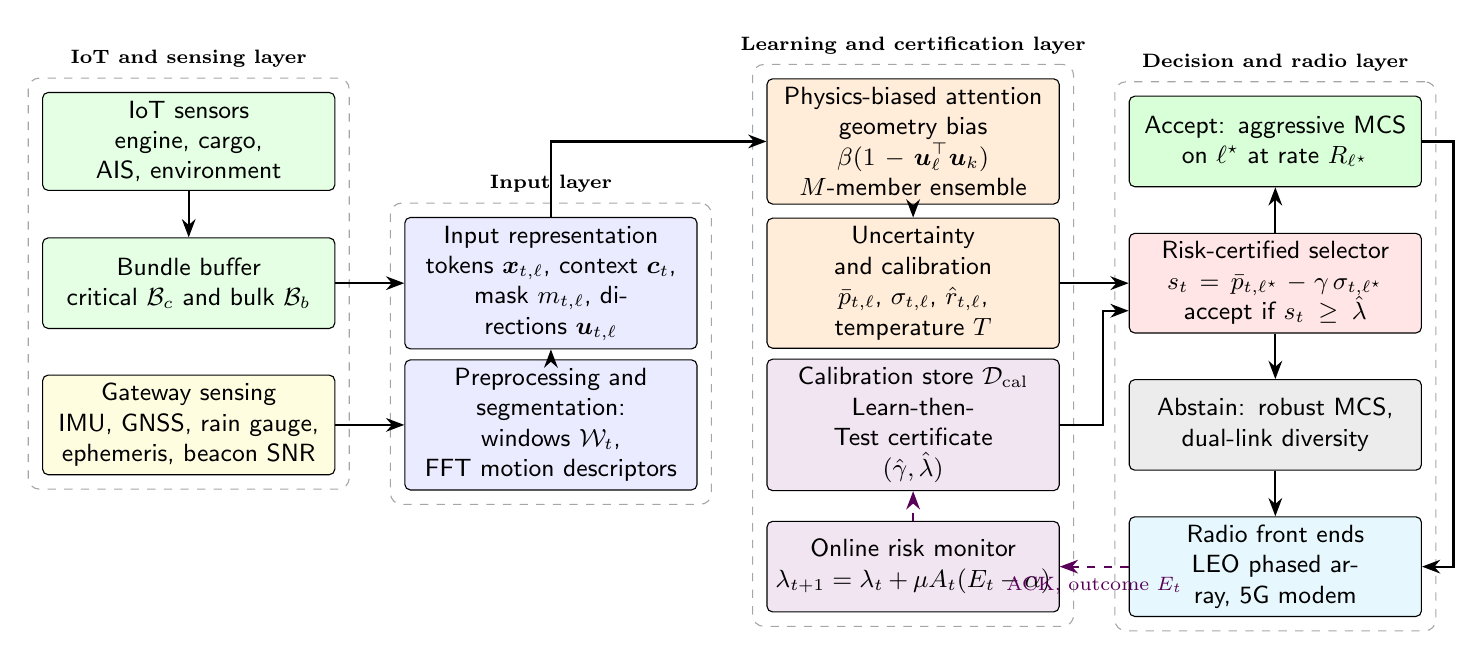
\begin{tikzpicture}[font=\sffamily\small, >=Stealth,
  b/.style={draw, rounded corners=2pt, align=center, minimum height=1.15cm, text width=3.5cm, fill=#1, inner sep=3pt},
  b/.default=white, ar/.style={->, thick}]
% column 1 (x=0): IoT and sensing
\node[b=green!10] (iot) at (0,4.2) {IoT sensors\\ engine, cargo, AIS, environment};
\node[b=green!10] (buf) at (0,2.4) {Bundle buffer\\ critical $\mathcal B_c$ and bulk $\mathcal B_b$};
\node[b=yellow!12] (sens) at (0,0.6) {Gateway sensing\\ IMU, GNSS, rain gauge,\\ ephemeris, beacon SNR};
% column 2 (x=4.6): input layer
\node[b=blue!8] (seg) at (4.6,0.6) {Preprocessing and\\ segmentation: windows $\mathcal W_t$,\\ FFT motion descriptors};
\node[b=blue!8] (tok) at (4.6,2.4) {Input representation\\ tokens $\bm x_{t,\ell}$, context $\bm c_t$,\\ mask $m_{t,\ell}$, directions $\bm u_{t,\ell}$};
% column 3 (x=9.2): learning and certification
\node[b=orange!15] (pba) at (9.2,4.2) {Physics-biased attention\\ geometry bias $\beta(1-\bm u_\ell^{\top}\bm u_k)$\\ $M$-member ensemble};
\node[b=orange!15] (unc) at (9.2,2.4) {Uncertainty and calibration\\ $\bar p_{t,\ell}$, $\sigma_{t,\ell}$, $\hat r_{t,\ell}$, temperature $T$};
\node[b=violet!10] (cal) at (9.2,0.6) {Calibration store $\mathcal D_{\rm cal}$\\ Learn-then-Test certificate\\ $(\hat\gamma,\hat\lambda)$};
\node[b=violet!10] (onl) at (9.2,-1.2) {Online risk monitor\\ $\lambda_{t+1}=\lambda_t+\mu A_t(E_t-\alpha)$};
% column 4 (x=13.8): decision and radio
\node[b=red!10] (sel) at (13.8,2.4) {Risk-certified selector\\ $s_t=\bar p_{t,\ell^\star}-\gamma\,\sigma_{t,\ell^\star}$\\ accept if $s_t\ge\hat\lambda$};
\node[b=green!15] (acc) at (13.8,4.2) {Accept: aggressive MCS\\ on $\ell^\star$ at rate $R_{\ell^\star}$};
\node[b=gray!15] (abs) at (13.8,0.6) {Abstain: robust MCS,\\ dual-link diversity};
\node[b=cyan!10] (rf) at (13.8,-1.2) {Radio front ends\\ LEO phased array, 5G modem};
% arrows
\draw[ar] (iot) -- (buf);
\draw[ar] (sens) -- (seg);
\draw[ar] (seg) -- (tok);
\draw[ar] (buf) -- (tok);
\draw[ar] (tok.north) |- (pba.west);
\draw[ar] (pba) -- (unc);
\draw[ar] (unc) -- (sel);
\draw[ar] (cal.east) -- ++(0.55,0) |- ($(sel.west)+(0,-0.35)$);
\draw[ar] (sel) -- (acc);
\draw[ar] (sel) -- (abs);
\draw[ar] (abs) -- (rf);
\draw[ar] (acc.east) -- ++(0.4,0) |- (rf.east);
\draw[ar, dashed, violet!70!black] (rf.west) -- node[below, font=\scriptsize] {ACK, outcome $E_t$} (onl.east);
\draw[ar, dashed, violet!70!black] (onl) -- (cal);
% layer frames
\begin{scope}[on background layer]
\node[draw=black!35, dashed, rounded corners, inner sep=5pt, fit=(iot)(buf)(sens)] (L1) {};
\node[draw=black!35, dashed, rounded corners, inner sep=5pt, fit=(seg)(tok)] (L2) {};
\node[draw=black!35, dashed, rounded corners, inner sep=5pt, fit=(pba)(unc)(cal)(onl)] (L3) {};
\node[draw=black!35, dashed, rounded corners, inner sep=5pt, fit=(sel)(acc)(abs)(rf)] (L4) {};
\end{scope}
\node[font=\scriptsize\bfseries, anchor=south] at (L1.north) {IoT and sensing layer};
\node[font=\scriptsize\bfseries, anchor=south] at (L2.north) {Input layer};
\node[font=\scriptsize\bfseries, anchor=south] at (L3.north) {Learning and certification layer};
\node[font=\scriptsize\bfseries, anchor=south] at (L4.north) {Decision and radio layer};
\end{tikzpicture}
\end{document}
